\chapter{Measurement Methodology}

This chapter is dedicated to answering the questions of what was measured and how results were obtained. Firstly, the GNU Radio flowgraphs are explained. Secondly, with reference to the flowgraphs measurement metrics are formally defined. Subsequently, the measurement setup is discussed in view of the necessity to verify the recorded data. Lastly, an overview of the semi-automatic measurement script system designed to automate, therefore accelerate the process of file system management, data processing and result plotting is given.

\bigskip

\section{GNU Radio Flowgraphs}

\subsection{Common Variables}

Our GNU Radio pure ALOHA and non-persistent/1-persistent CSMA implementations are placed on top of a common PHY layer warranting comparability. The specific PHY layer implementation is beyond this work's scope, but a few parameters common to all flowgraphs shall be discussed nonetheless. Hereinafter, these variables and their values will not be mentioned unless they are important concerning the interpretation of results.

\begin{figure}[ht]
	\label{fig:grc-common-variables}
	\begin{center}
		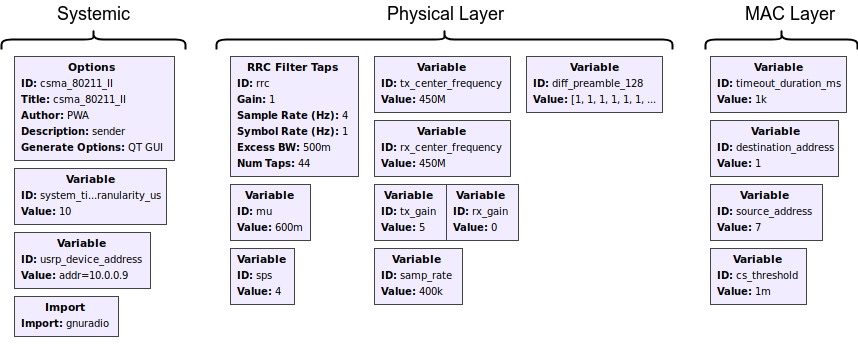
\includegraphics[width=\textwidth]{pictures/grc_common_variables}
	\end{center}
\caption{Variables Common to All Flowgraphs}
\end{figure}     

\subsection{Receiver and Sniffer}

\begin{sidewaysfigure}[ht]
	\label{fig:grc-receiver}
	\begin{center}
		\subfloat[Receiver]{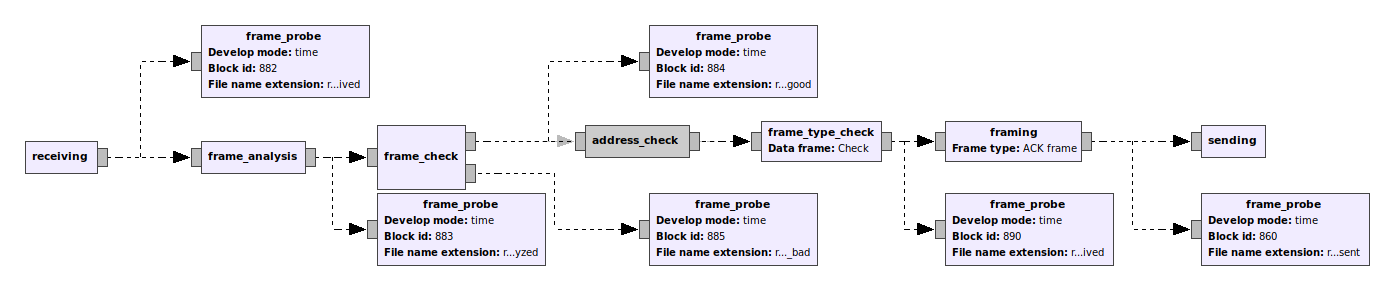
\includegraphics[width=\textwidth]{pictures/grc_receiver_flowgraph}}
		\vskip 40pt
		\subfloat[Sniffer]{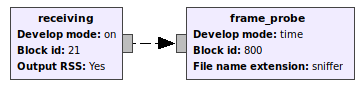
\includegraphics[width=0.3\textwidth]{pictures/grc_sniffer_flowgraph}}
	\end{center}
	\caption{GRC Receiver Flowgraphs}
\end{sidewaysfigure}

\subsection{Pure ALOHA Transmitter}

\begin{sidewaysfigure}[h]
	\label{fig:grc-aloha-sender}
	\begin{center}
		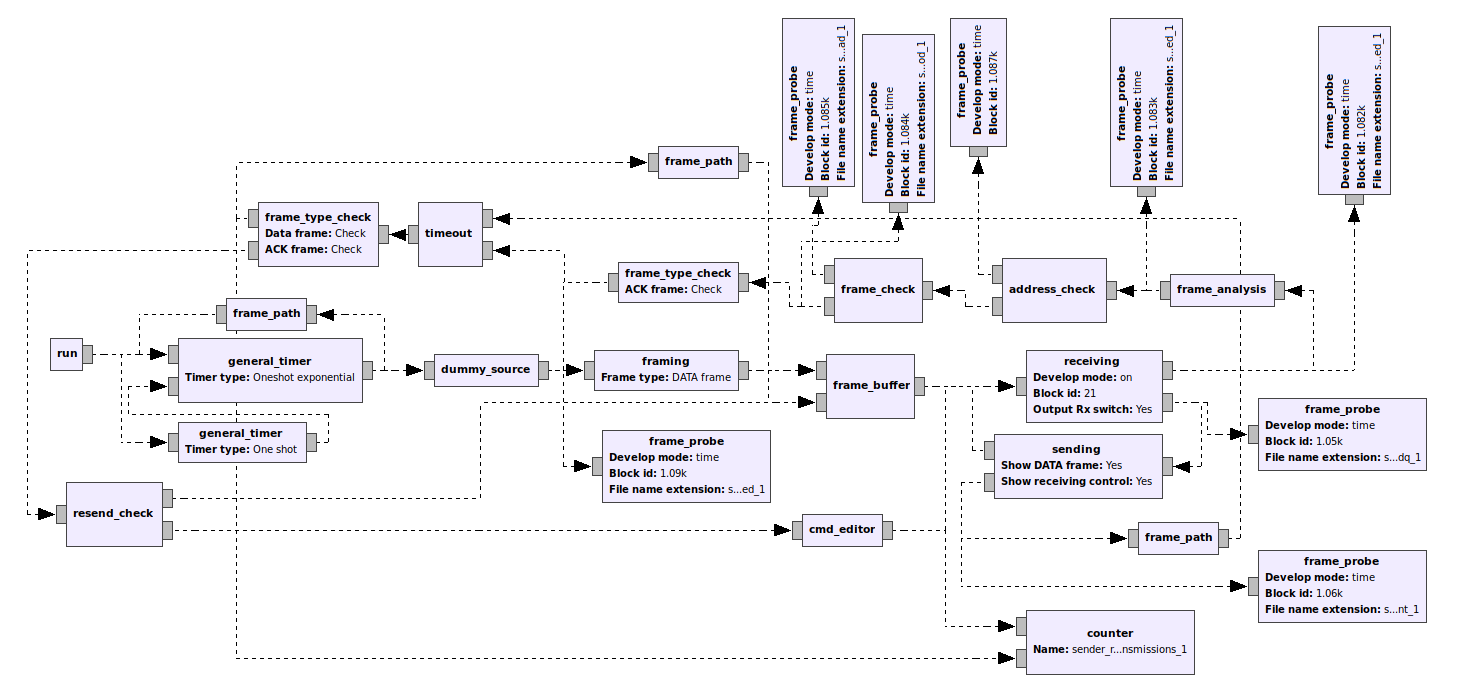
\includegraphics[width=\textwidth]{pictures/grc_aloha_transmitter_flowgraph}
\end{center}
\caption{GRC Pure ALOHA Transmitter Flowgraph}
\end{sidewaysfigure}

\subsection{CSMA Transmitter}

\begin{sidewaysfigure}[h]
	\label{fig:grc-csma-sender}
	\begin{center}
		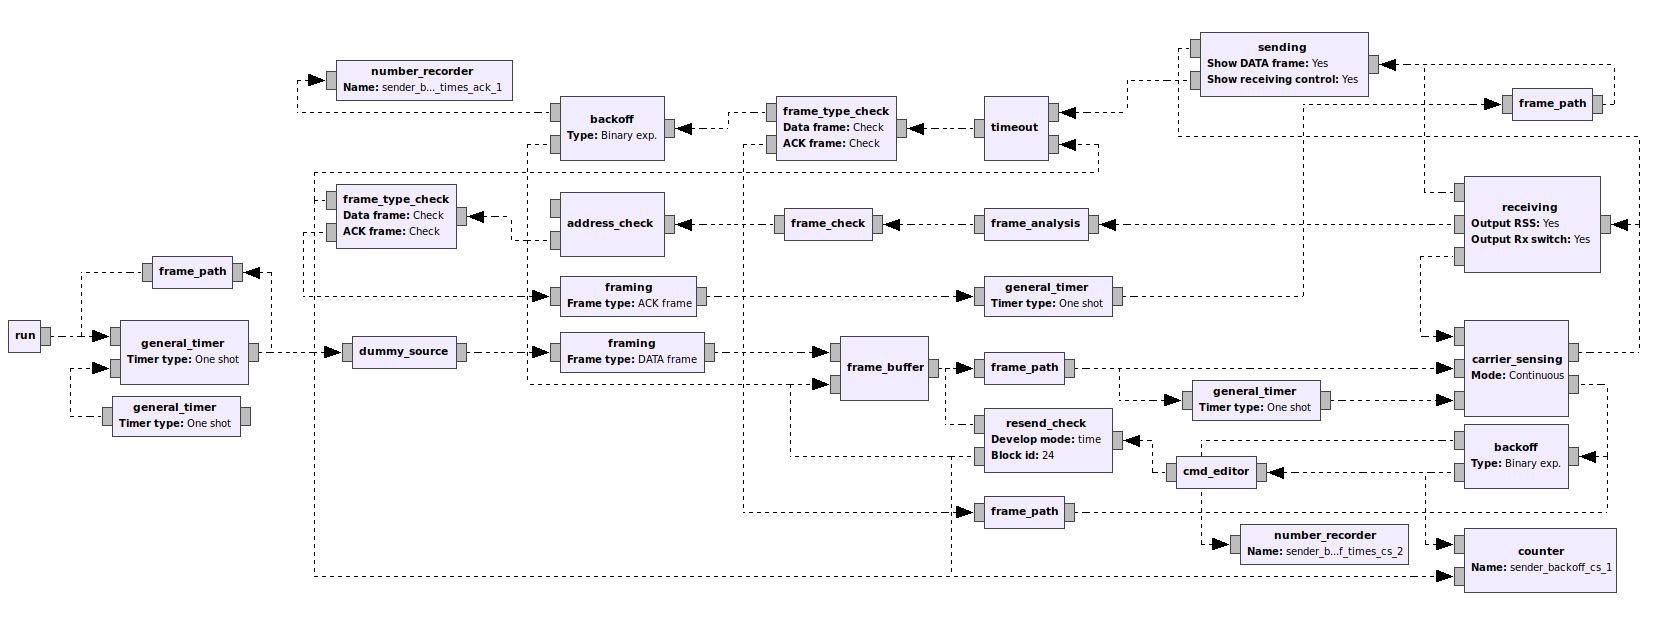
\includegraphics[width=\textwidth]{pictures/grc_csma_transmitter_flowgraph}
\end{center}
\caption{GRC CSMA Transmitter Flowgraph}
\end{sidewaysfigure}

\subsection{Sniffer}

\section{Measurement Metrics}

\section{Measurement Setup}

\begin{figure}[ht]
	\label{fig:measurement-setup}
	\begin{center}
		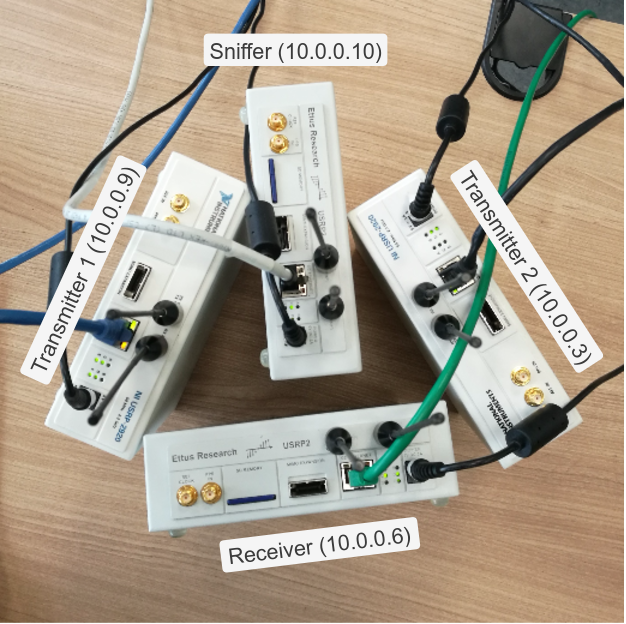
\includegraphics[width=0.5\textwidth]{pictures/measurement_setup}
	\end{center}
	\caption{Photo of the Measurement Setup}
\end{figure}

\section{Measurement Script System}
\label{sec:script-system}

\begin{figure}[ht]
	\label{fig:script-system}
	\begin{center}
		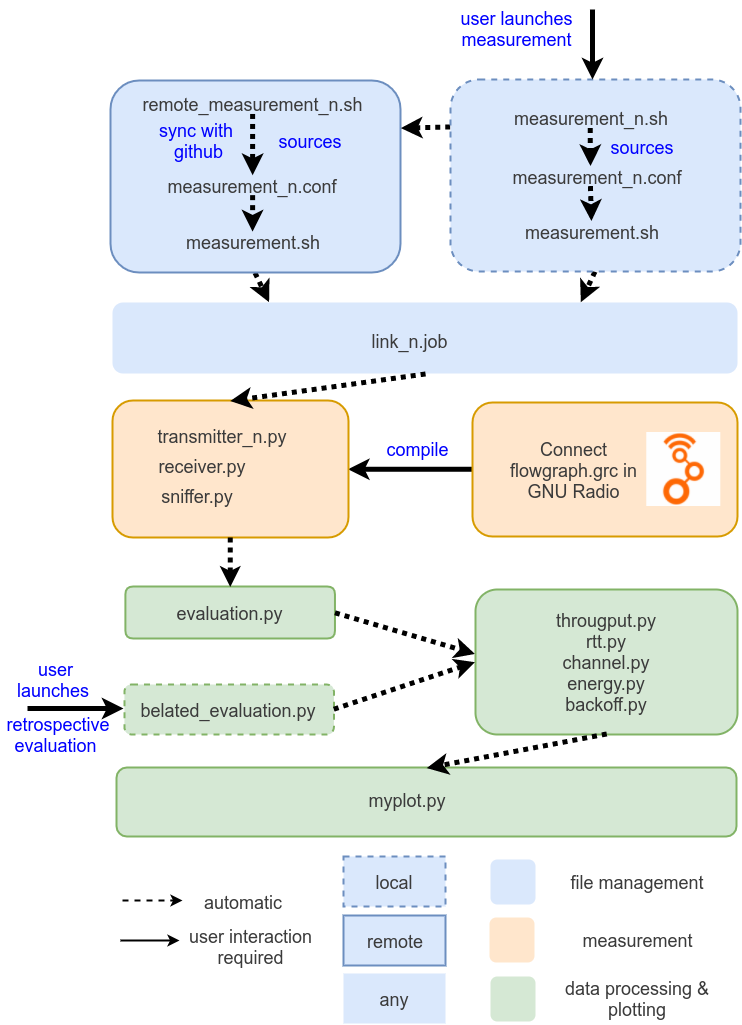
\includegraphics[width=0.6\textwidth]{pictures/script_system}
	\end{center}
	\caption{The Three-Phase Measurement Script System}
\end{figure}